\documentclass{article}[a4paper,12pt]
\usepackage[utf8]{inputenc}
\usepackage{amsmath,amssymb,amsthm,amsfonts,mathtools}
\usepackage[inline]{enumitem}
\usepackage{soul}
\usepackage{cancel}
\usepackage{hyperref}
\usepackage{centernot}
\usepackage{pifont}
\usepackage{changepage}
\usepackage{subcaption}
\usepackage[section]{placeins}
\usepackage{lipsum, graphicx, caption}
\usepackage{float}
\usepackage{commath}
\usepackage{wrapfig}
\usepackage{amsmath}
\usepackage{amsfonts}
\usepackage{amssymb}
\usepackage{fancyvrb}
\fvset{tabsize=4}
\theoremstyle{definition}
\newtheorem{innercustomgeneric}{\customgenericname}
\providecommand{\customgenericname}{}
\newcommand{\newcustomtheorem}[2]{%
  \newenvironment{#1}[1]
  {%
   \renewcommand\customgenericname{#2}%
   \renewcommand\theinnercustomgeneric{##1}%
   \innercustomgeneric
  }
  {\endinnercustomgeneric}
}
\newcustomtheorem{customthm}{Theorem}
\newcustomtheorem{customlem}{Lemma}
\newcustomtheorem{customdefn}{Definition}
\newcustomtheorem{customprop}{Proposition}
\newcustomtheorem{customexer}{Exercise}
\renewcommand{\qedsymbol}{$\blacksquare$}

\newcommand{\Lagr}{\mathcal{L}}

\setlength\parindent{0pt}
\let\emptyset\varnothing
\usepackage{geometry}
\geometry{
	a4paper, portrait,
	total = {170mm,257mm},
	left = 20mm,
	top = 20mm,
}

\usepackage{xcolor}
\usepackage{pagecolor}
\pagecolor{white}
\color{black}

\title{\textbf{Neural Networks and Deep Learning}}
\author{
	\textbf{Om Prabhu}\\
	19D170018\\
	Undergraduate, Department of Energy Science and Engineering\\
	Indian Institute of Technology Bombay\\}
\date{Last updated \today}

\begin{document}
\maketitle
\vspace{-12pt}
\hrulefill
\vspace{6pt}

\textbf{NOTE:} This document is a brief compilation of my notes taken during the course `Neural Networks and Deep Learning'. You are free to use it and my project files for your own personal use \& modification. You may check out the course and/or specialization here: \texttt{\href{https://www.deeplearning.ai/}{deeplearning.ai}}.

\hrulefill
\tableofcontents
\vspace{6pt}

\hrulefill
\pagebreak

\section{Introduction}
\subsection{About myself}
Hello. I am Om Prabhu, currently an undergrad at the Department of Energy Science and Engineering, IIT Bombay. If you have gone through my website (\texttt{\href{https://omprabhu31.github.io/}{https://omprabhu31.github.io/}}) earlier, which is probably where you found this document too, you will know that I am quite a bit into programming and tinkering with code to try and do cool stuff. Additionally, I love playing video games, listening to music and engaging in a little bit of creative writing as and when I get time. With this brief self-introduction, let us get into why I decided to pursue this course.
\subsection{A little bit about deep learning}
As you probably know, deep learning has already transformed traditional internet businesses like web search and advertising. Further, it is also helping in the creation of businesses and business products and even jobs. Deep learning is making it into almost all types of industries ranging from healthcare and medical diagnosis to personalized education, precision agriculture and many others. 
\vspace{6pt}

Just as how electricity once transformed countless industries, AI today is on its way to doing the same. The part of AI that is contributing to most of this transformation is deep learning. This is a technical course which will teach us how to build neural networks and by the end of this course, we will be able to build a cat recognizer (for some reason, there is this cat meme running around in the world of AI which will also be discussed later).

\hrulefill
\pagebreak
\section{Overview of Deep Learning}
The terminology in AI is still not very well defined. For example, some people say that neural networks are a subset of deep learning while others use the two words almost interchangeably. Through most of these notes, we will refer to deep learning as being a science of building and training neural networks. With that said, let's look at what a neural network is.
\subsection{Neural networks}
Let us use an example of demand prediction to try and understand what neural networks really are. Suppose a t-shirt company wants to know how many units they can expect to sell based on their selling price. The required dataset might be a in the form of a demand curve, where the higher the price the lesser the demand. This form of curve can be used to train what is perhaps the simplest possible neural network.
\begin{center}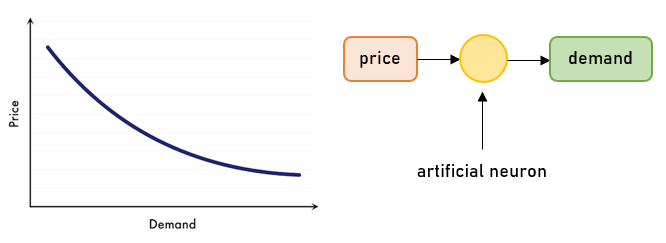
\includegraphics{deep_learning1.png}\end{center}
All this single-neuron network does is compute the curve shown and `learn' it in order to map any value of price to the appropriate value of demand. A single neuron can be thought of as a Lego brick, and a neural network as a very complicated stack, often in multiple layers, of such bricks.
\vspace{6pt}

Let's look at a more complicated example. Suppose that instead of just the price, we have more variables like shipping cost, marketing cost and material. Then we will have multiple factors that influence demand like affordability, consumer awareness and perceived quality. We might then have a slightly more complicated neural net like the one below:
\begin{center}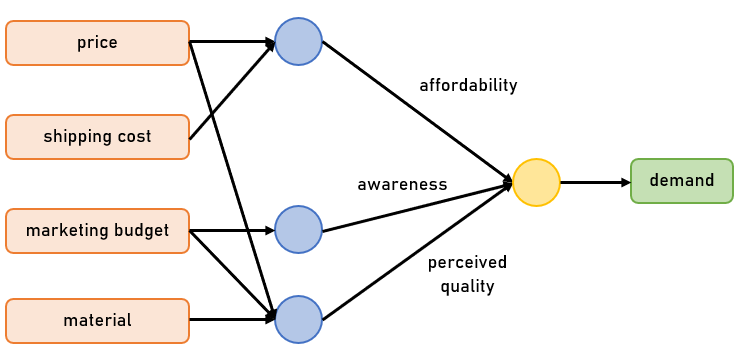
\includegraphics{deep_learning2.png}\end{center}
This slightly more complicated neural network maps the 4 input parameters to the output that is the demand.
\vspace{6pt}

From that the way in which we have discussed neural networks above, it appears as if we have to actually figure out the key factors as affordability, awareness and perceived quality. However, things do not work this way. One of the best things about neural networks is that we only have to provide it the input and the output $-$ all of the stuff in the middle, it figures out by itself. It automatically `learns' and completely trains itself to find the most accurate possible function that maps from the input to the output.
\vspace{6pt}

Another little correction is that it seems like the first node takes in only price and shipping inputs and so on. This is not the case. In practice, all nodes will be fed in with all the inputs and we let the individual neurons decide how many inputs they want to use and how they use them.
\subsection{Supervised learning with neural networks}
Most of the value created through deep learning has been in applications of supervised learning. This is the task of learning a function that maps an input to an output based on example input-output pairs (or A $\rightarrow$ B mapping). This has turned out to be very profitable for many industries such as:
\begin{itemize}
	\item online advertising: input is ad \& user info using which the algorithm tries to figure out if the user is likely to click on the ad
	\item computer vision: this is a very vast application area of AI (for example, input is an image and the algorithm tries to figure out whether the image is part of a dataset of 1000 images)
	\item speech recognition: input an audio clip and output a text transcript based on the input
	\item machine translation: input text or documents in certain languages and receive a translated output
	\item autonomous driving: AI algorithm uses image \& sensor info to figure out the position of nearby cars so it can avoid them
\end{itemize}
It turns out that slightly different types of neural networks are useful for different applications. For example, convolutional neural networks (CNN) are most commonly used for image applications while recurrent neural networks (RNN) are better for processing sequential data such as audio. More complicated applications often require the generation of custom neural network architecture.
\begin{center}
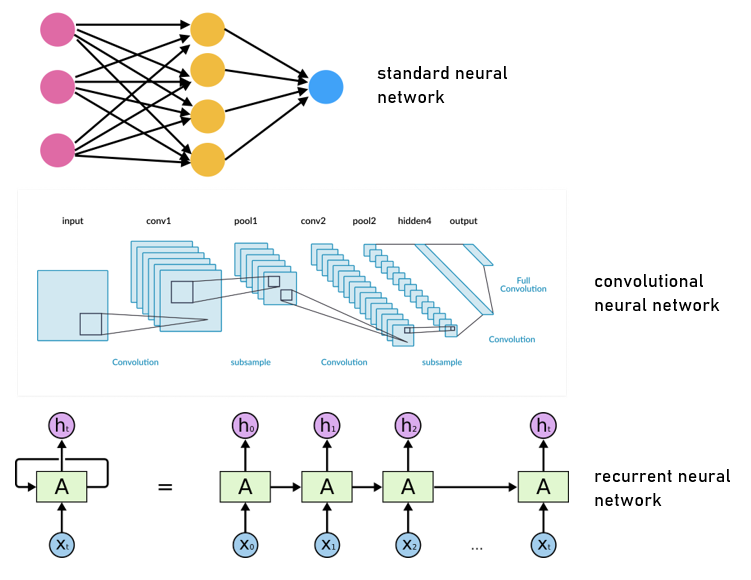
\includegraphics{types_of_nn.png}
\end{center}
Finally, supervised learning can be applied to both structured data (highly organized data such as tables, spreadsheets and databases) as well as unstructured data (data in the form of images, audio, video and even raw text).
\subsection{Why is deep learning taking off now?}
The ideas for deep learning and neural networks have been around for decades. Why is it that they have taken off only recently?
\vspace{6pt}

One of the major drivers of deep learning is scale. This refers to the ability of technology to train large sets of neural networks to process huge amounts of data while also improving AI performance. This can be illustrated through a graph as follows:
\begin{center}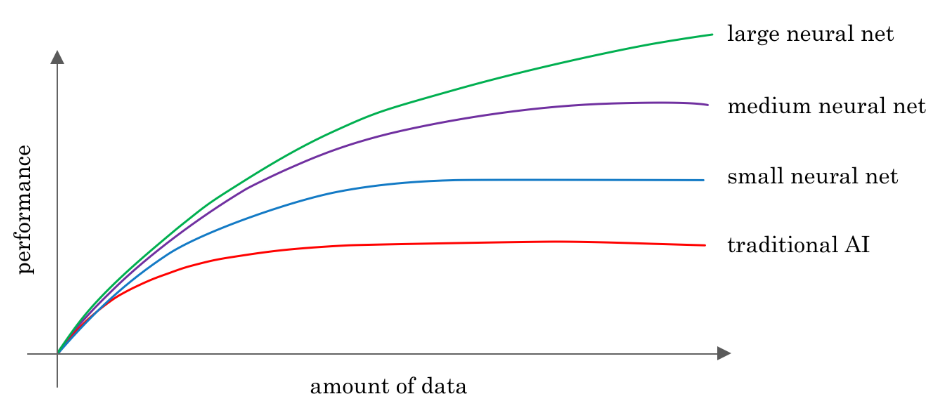
\includegraphics[scale=0.65]{data_vs_performance.png}\end{center}
\begin{itemize}
	\item for traditional deep learning systems, the data vs performance graph maxes out pretty early
	\item on training increasingly complex neural networks with higher amounts of data, performance keeps on getting better for much longer  
\end{itemize}
Hence to achieve the highest performance levels, we need two things. Firstly, it helps to have a lot of data. Additionally, we need the ability to train large sets of neural networks. Earlier, it was almost as if AI systems didn't know what to do with huge amounts of data. Now, with fast \& powerful CPUs and GPUs, it is possible for us to train large neural networks with a high amount of data.
\vspace{6pt}

Another factor is that of algorithmic innovation in order to increase the training speeds of neural networks. One of the major breakthroughs in this area has been the switch from sigmoid functions to ReLU functions:
\begin{center}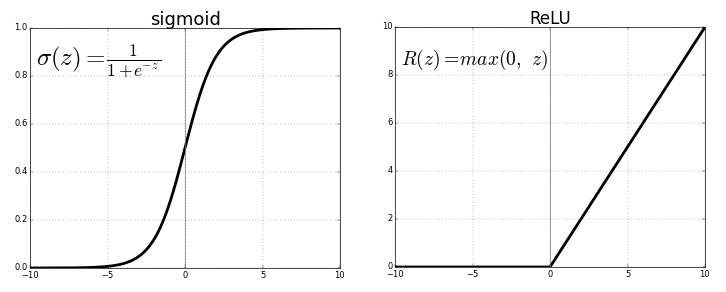
\includegraphics[scale=0.5]{sigmoid_relu.png}\end{center}
It turns out that on the tapering ends of the sigmoid function, since the gradient is nearly zero, the parameters hardly change and the training becomes very slow. In a ReLU curve, the gradient does not gradually shift to zero, so there is no point where the learning speed of the network is very slow. 
\vspace{6pt}

Fast computation is very important in deep learning, since the idea of training a neural network involves a lot of iterating $-$ basically we input the data, then train the neural network, then get feedback about how well the neural network performed, and then make changes to the data and neural network and repeat the cycle over and over until the neural network is trained well enough. Hence by reducing computation speeds, it leads to a huge rise in productivity while building out neural networks for AI projects.

\hrulefill
\begin{center}\textbf{END OF WEEK 1}\end{center}
This is the end of the course notes for Week 1. Keep on reading further for notes from further weeks, or spend some time gaining further insight into the previously discussed topics.

\hrulefill
\pagebreak
\section{Logistic Regression as a Neural Network}
Now that we have an idea of what neural networks are and what they can do, let us dive into the basics of neural network programming. Many of these ideas can be discussed using the concept of logistic regression.
\vspace{6pt}

\textbf{NOTE:} Throughout the document, there will be extensive use of the following notation:
\begin{enumerate}
	\item a single input feature vector has dimension $n_x$
	\item a single training example is represented by $(x,y)$ $\rightarrow$ $x\in\mathbb{R}^{n_x},$ $y\in\{0,1\}$
	\item a training set comprises $m$ (or $m_{train}$) training examples, i.e. $\{(x^{(1)},y^{(1)}), (x^{(2)},y^{(2)}), \dots, (x^{(m)},y^{(m)})\}$
	\item a test set similarly contains $m$ (or $m_{test}$) test examples
	\item to put all training examples $x$ into a more compact notation, we define a matrix $X\in\mathbb{R}^{n_x\times m}$ as follows:
\begin{center}
$X$ = 
$\begin{bmatrix}
	\vdots & \vdots & & \vdots\\
	x^{(1)} & x^{(2)} & \cdots & x^{(m)}\\
	\vdots & \vdots & & \vdots\\
\end{bmatrix}$
\end{center}
	\item to put all output labels $y$ into a more compact notation, we define a matrix $Y\in\mathbb{R}^{1\times m}$ as follows:
\begin{center}
$Y$ = 
$\begin{bmatrix}
	y^{(1)} & y^{(2)} & \cdots & y^{(m)}\\
\end{bmatrix}$
\end{center}
	\item terms of the form $x^{(i)}$, $y^{(i)}$, etc are associated with the $i^{th}$ training example
\end{enumerate}
\subsection{Derivatives (optional)}
Throughout this document, there will be a lot of differential calculus (i.e. the calculus of derivatives). Let us get somewhat familiar with derivatives before we move on to other concepts. This is by no means a comprehensive guide on differential calculus, for which you may look through some of the resources at the end of this section.

\begin{wrapfigure}[13]{L}{0.3\textwidth}
\centering 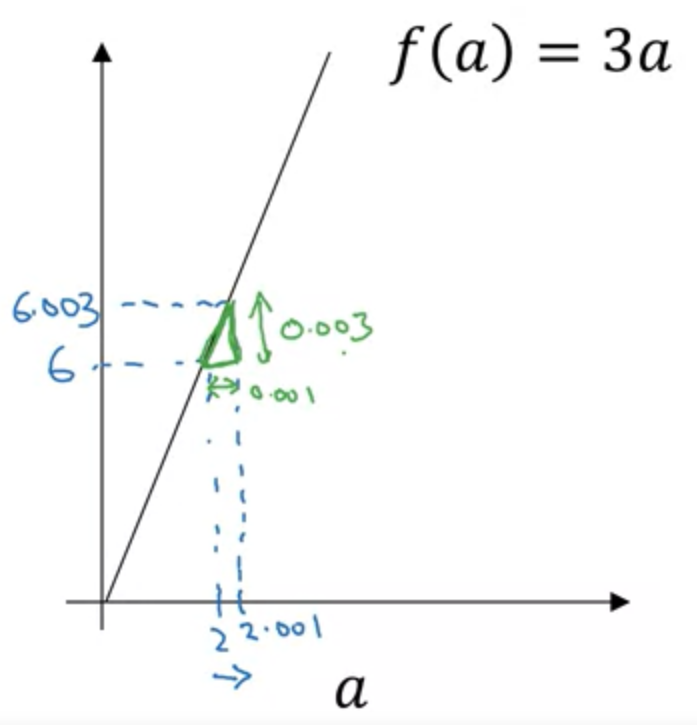
\includegraphics[width=0.28\textwidth]{y_equals_3x.png}
\end{wrapfigure}
\vspace{6pt}

Consider this simple function $f(a)=3a$. Let $a=2$, then $f(a)=6$. Let's now change $a$ by a very small amount, maybe $a=2.001$. Then we get $f(a)=6.003$.
\vspace{6pt}

Now if we construct a triangle as in the diagram, we see that `nudging' $a$ to the right by $0.001$ causes $f(a)$ to increase by $0.003$. For each 1 unit of change in $a$, there is a corresponding change of 3 units in $f(a)$. 
\vspace{6pt}

We say that the slope, or derivative, of the function $f(a)$ is 3. More specifically, it is the derivative of the function with respect to $a$ at $a=2$. More formally, we define the derivative of a function at a specific point as the rate of change of the function value at that point. Mathematically, we can write this as
$$\frac{\text{d}f(a)}{\text{d}a}=3=f^{\prime}(a)$$

\begin{wrapfigure}[10]{R}{0.31\textwidth}
\centering 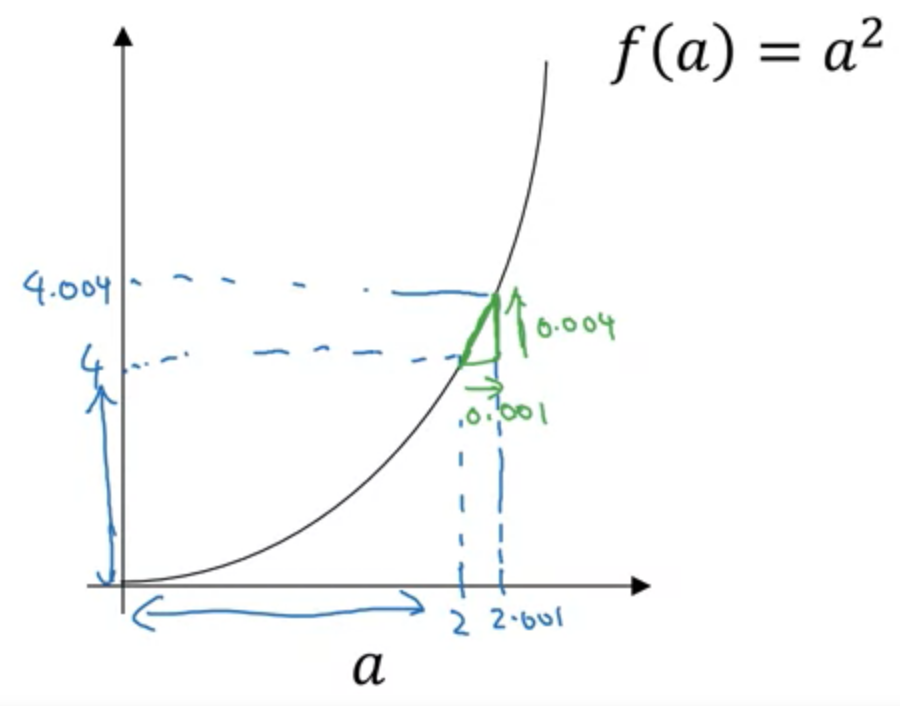
\includegraphics[width=0.31\textwidth]{x_square.png}
\end{wrapfigure}
\vspace{6pt}

The function represented above is a typical linear function $-$ its derivative at any point along the function is constant. Let us take a more complicated example, $f(a)=a^2$. At $a=2$, $f(a)=4$. Now, on changing $a=2.001$, we get $f(a)=4.004001\approx4.004$. 
\vspace{6pt}

Constructing a similar triangle, we can conclude that the slope of the function at $a=2$ is 4. What about at $a=5$?
\vspace{6pt}

At $a=5$, $f(a)=25$ while at $a=5.001$, $f(a)=25.010001\approx 25.01$. Again by a quick computation, the slope of the function at $a=5$ comes out to be 10.
\vspace{6pt}

As it happens, the derivative of the function $f(a)=a^2$ at any given point on the function is $2a$. 

\vspace{6pt}

This description of derivatives might make it look like they are an approximation, but this is not the case. In practice, the amount by which $a$ is changed is infinitesimally small, which gives rise to another concept in calculus known as limits (will not be discussed here). 
\pagebreak

If you wish to know more about derivatives and/or limits, feel free to go through the resources listed below. A expertise in differential calculus is not desired, but a working knowledge always helps: 
\begin{itemize}
	\item \texttt{\href{https://www.khanacademy.org/math/calculus-1/cs1-limits-and-continuity}{Limits and Continuity (by Khan Academy)}}
	\item \texttt{\href{https://www.khanacademy.org/math/calculus-1/cs1-derivatives-definition-and-basic-rules}{Derivatives: Definition and Basic Rules (by Khan Academy)}}
	\item \texttt{\href{https://www.khanacademy.org/math/calculus-1/cs1-derivatives-chain-rule-and-other-advanced-topics}{Derivatives: Chain Rule and Other Advanced Topics (by Khan Academy)}}
	\item \texttt{\href{https://www.khanacademy.org/math/calculus-1/cs1-applications-of-derivatives}{Application of Derivatives (by Khan Academy)}}
	\item \texttt{\href{http://www-math.mit.edu/~djk/calculus_beginners/}{Calculus for Beginners - MIT Mathematics}}
	\item \texttt{\href{https://ocw.mit.edu/resources/res-18-001-calculus-online-textbook-spring-2005/textbook/}{Online Calculus Textbook - MIT OpenCourseWare}}
	\item \texttt{\href{https://math.stackexchange.com/questions/tagged/calculus}{Mathematics StackExchange - Tags (Calculus)}}
\end{itemize}

\subsection{Binary classification}
Logistic regression is an algorithm for binary classification. An example of binary classification is taking in an input of an image and classifying it as a cat or not a cat. Let's look at how images are represented in computers.
\vspace{6pt}

Humans perceive images by their subtle features. A computer looks at an image as an array of pixels. A computer stores 3 separate matrices, each the size of the pixel map (i.e. 1920$\times$1080, 1024$\times$768, etc), corresponding to the RGB channels of the image. To process images, a computer `unpacks' the pixel intensity values to create what is known as a feature vector. 

\begin{wrapfigure}[7]{L}{0.5\textwidth}
\centering 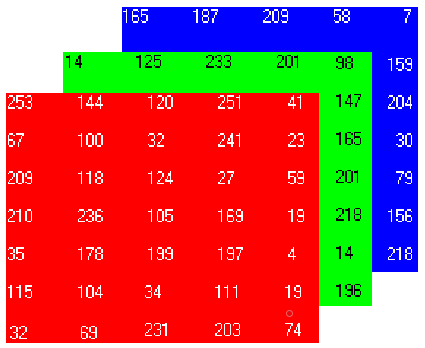
\includegraphics[width=0.48\textwidth]{rgb_matrices.png}
\end{wrapfigure}

We just take all the red pixel values and list them one by one, followed by the green pixel values and then the blue pixel values, as shown below:
\begin{center}
$x$ =
$\begin{bmatrix}
	253\\
	144\\
	\vdots\\
	14\\
	125\\
	\vdots\\
	165\\
	187\\
	\vdots\\
\end{bmatrix}$
\end{center}
Suppose we have a 64$\times$64 image. The resulting feature vector will have 64$\times$64$\times$3 (12288) dimensions.
\vspace{-6pt}

We usually use $n_x$ (sometimes $n$ for convenience to represent the dimensions of the input feature vector $x$. Our goal in binary classification is to input a $n_x-$dimensional feature vector corresponding to a pixel map and output either a 0 or 1. 
\subsection{Logistic regression}
Logistic regression is an algorithm where the output labels $y$ in a supervised learning problem are all either 0 or 1 (i.e. for binary classification problems).
\vspace{6pt}

Let us continue with the earlier example of classifying images of cats. Given an input feature vector $x$, we want an algorithm to output an estimate $\hat{y}$ of $y$ (i.e. the chance that $y=1$ given the input image). More formally, 
\begin{center}
Given $x$, want $\hat{y}$ = $P(y=1\mid x)$
\end{center}
Given that $x\in\mathbb{R}^{n_x}$, the parameters of the logistic regression will be $w\in\mathbb{R}^{n_x}$, $b\in\mathbb{R}$. So given an input $x$ and the parameters $w$ \& $b$, how do we generate the output $\hat{y}\in\mathbb{R}$? 
\vspace{6pt}

One thing we could try (that doesn't work) is letting $\hat{y}=w^Tx+b$. This is, in fact, what we do in linear regression. This doesn't work for binary classification because we want $\hat{y}$ to be the chance that $y=1$, i.e. $\hat{y}\in\left[0,1\right]$. Since the range of $w^Tx$ is not definite, it is very difficult to enforce the restrictions on $\hat{y}$.

\begin{wrapfigure}[9]{L}{0.4\textwidth}
\centering 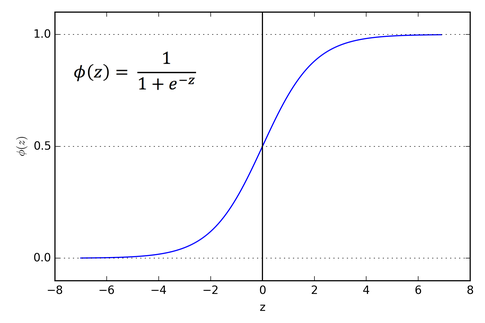
\includegraphics[width=0.38\textwidth]{sigmoid_logistic_regression.png}
\end{wrapfigure}
\vspace{6pt}

Instead what we do in logistic regression is $\hat{y}=\sigma(w^Tx+b)$, where $\sigma$ is the sigmoid function (shown in the diagram alongside, ignore the $\phi(z)$ notation). Defining $z=w^Tx+b$,
\begin{center}
$\boxed{\sigma(z)=\dfrac{1}{1+e^{-z}}}$
\end{center}
If $z$ is a large positive number, $e^{-z}\rightarrow 0$, $\therefore\sigma(z)\rightarrow 1$

If $z$ is a large negative number, $e^{-z}\rightarrow \infty$, $\therefore\sigma(z)\rightarrow 0$
\vspace{6pt}

We have now seen the logistic regression model in quite a bit of detail. However, to train the parameters $w$ and $b$, we need to define a cost function.
\subsection{Cost function in logistic regression}
To train the parameters of our logistic regression model, we have a training set of $m$ training examples. Given $\{(x^{(1)},y^{(1)}), (x^{(2)},y^{(2)}), \dots, (x^{(m)},y^{(m)})\}$, we want to find parameters $w$ and $b$ so that $\hat{y}^{(i)}\approx y^{(i)}$. To recap, $$\hat{y}^{(i)}=\sigma(z^{(i)})=\dfrac{1}{1+e^{-z^{(i)}}}\text{ where }z^{(i)}=w^Tx^{(i)}+b$$
Let us now see a loss/error function we can use to measure how well our algorithm is doing. One thing we could do (that, again, doesn't work) is define $\Lagr(\hat{y},y)=\dfrac{1}{2}(\hat{y}-y)^2$. In practice, this leads to the optimization becoming non-convex (i.e. we end up with multiple local optima), so gradient descent (discussed in the next section) may not find the global optimum.
\vspace{6pt}

Instead, we define a different loss function to get a convex optimization problem. 
$$\boxed{\Lagr(\hat{y},y)=-(y\log\hat{y}+(1-y)\log(1-\hat{y}))}$$
On first sight, it seems this function was conjured from thin air. Here's some intuition for why it makes sense. If we use a squared error, then we would want the squared error to be as small as possible. Similarly, we also want the above loss function to be as small as possible. Let's look at 2 cases: 
\begin{itemize}
	\item if $y=1$: $\Lagr(\hat{y},y)=-\log\hat{y}\implies$ $\log\hat{y}$ to be large $\implies$  $\hat{y}$ to be large
\end{itemize}
But since $\hat{y}$ is a sigmoid function, it is always $\leqslant 1$. Hence, if $y=1$, we want $\hat{y}$ to be as close to 1 as possible.
\begin{itemize}
	\item if $y=0$: $\Lagr(\hat{y},y)=-\log(1-\hat{y})\implies$ $(1-\log\hat{y})$ to be large $\implies \log\hat{y}$ to be small $\implies \hat{y}$ to be small
\end{itemize}
But $\hat{y}$ can never be smaller than 0. Hence, if $y=0$, we want $\hat{y}$ to be as close to 0 as possible. One may argue that there are many such functions which roughly satisfy the 2 conditions above. We will discuss later why we choose a loss function with this particular form.
\vspace{6pt}

Finally, the loss function above is designed with respect to a single training example, i.e. it measures how well our algorithm is doing on a single example. Now let us define the cost function, which measures how well our algorithm is doing on the entire training set.
\vspace{6pt}

The cost function $J$, which is applied to parameters $w$ \& $b$, is just the simple average of the loss function applied to each of the training examples.
$$\boxed{J(w,b)=\dfrac{1}{m}\sum_{i=1}^{m}\Lagr(\hat{y}^{(i)},y^{(i)})=-\dfrac{1}{m}\sum_{i=1}^{m}\left[y^{(i)}\log\hat{y}^{(i)}+(1-y^{(i)})\log(1-\hat{y}^{(i)})\right]}$$
Using this, we try to find parameters $w$ \& $b$ that minimize the overall costs function $J$. 
\subsection{Gradient descent}
Up till now, we've seen the logistic regression model, the loss and cost functions for the parameters of the algorithm. Let us now see how the gradient descent algorithm can be used to train the parameters $w$ \& $b$ on a training set. From the previous section, we have the cost function
$$J(w,b)=\dfrac{1}{m}\sum_{i=1}^{m}\Lagr(\hat{y}^{(i)},y^{(i)})=-\dfrac{1}{m}\sum_{i=1}^{m}\left[y^{(i)}\log\hat{y}^{(i)}+(1-y^{(i)})\log(1-\hat{y}^{(i)})\right]$$
We naturally want to find $w, b$ that minimize $J(w,b)$. We do this using what is known as the gradient descent algorithm. Here's an illustration of gradient descent.
\begin{wrapfigure}[10]{R}{0.4\textwidth}
\centering 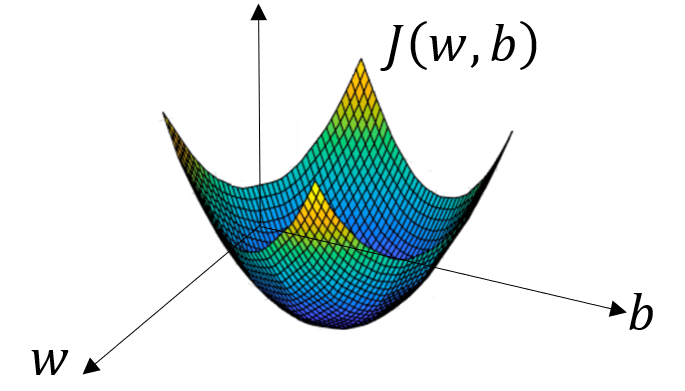
\includegraphics[width=0.38\textwidth]{gradient_descent.png}
\end{wrapfigure}
\vspace{6pt}

Note that, in practice, $w$ is of a much higher dimension, but for illustrative purposes let's assume it is a single real number. As seen, $J(w,b)$ has a single global optimum, and we want to find $w,b$ corresponding to this minimum.
\vspace{6pt}

To do this, we first initialize $w$ \& $b$ to some value (for convenience, we usually initialize them both to 0).
\vspace{6pt}

After this, what the gradient descent algorithm does is take a step in the steepest downhill direction. There can multiple iterations of the gradient descent cycle until the point the algorithm decides that it has reached the global optimum. 
\vspace{6pt}

This gives us a brief overview of how gradient descent works. Let's dive deeper into the details. Consider a one-dimensional plot with only $w$ as the parameter.
\begin{wrapfigure}[9]{L}{0.4\textwidth}
\centering 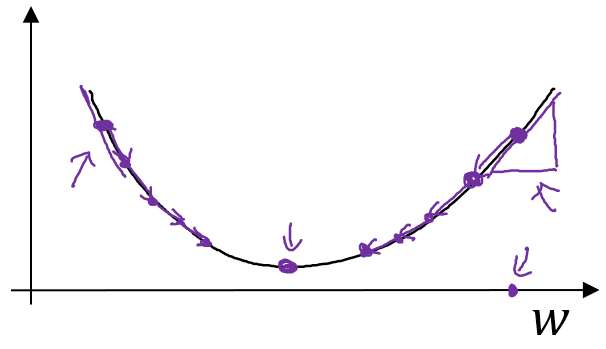
\includegraphics[width=0.38\textwidth]{1d_convex_plot.png}
\end{wrapfigure}
\vspace{6pt}

The gradient descent algorithm repeatedly carries out the following update until it converges to the global optimum value:
$$w\equiv w-\alpha\left(\frac{\text{d}J(w)}{\text{d}w}\right)$$
where $\alpha$ is the learning rate, which controls how big each step in the gradient descent is. 
\vspace{6pt}

No matter where we initialize the value of $w$, the gradient descent algorithm will always reach the global optimum at some point. 
\vspace{6pt}

Since we actually have a function $J$ in 2 parameters, the loop of gradient descent becomes as follows:
$$w\equiv w-\alpha\left(\frac{\partial J(w,b)}{\partial w}\right)\text{; } b\equiv b-\alpha\left(\frac{\partial J(w,b)}{\partial b}\right)$$
When we actually get down to coding such and algorithm, we will use the following (mathematically inconsistent) notation:
$$\text{d}w\equiv \frac{\partial J(w,b)}{\partial w} \text{; } \text{d}b\equiv \frac{\partial J(w,b)}{\partial b}\longrightarrow w\equiv w-\alpha\text{d}w; b\equiv b-\alpha\text{d}b$$ 
\subsection{Computation graph}
The computations of a neural network are organized in terms of a forward pass, in which we compute the output of the neural network, and a backward pass, in which we compute the derivatives. The computation graph explains why it is organized this way. To illustrate it, let's take a very simple example.
\vspace{6pt}

Let's say we want to compute a function $J(a,b,c)=3(a+bc)$. There are 3 steps involved in computing this function. First, we compute the value of $bc$ and maybe store that in a variable $u$. Then we compute $v=a+u$ and finally, we compute $J=3\times v$. We might construct a computation graph that might look like the one below.
\begin{wrapfigure}[6]{L}{0.4\textwidth} 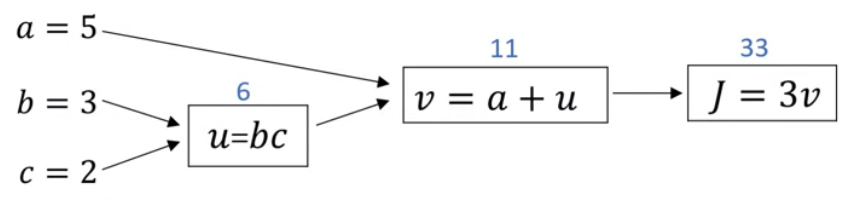
\includegraphics[width=0.4\textwidth]{computation_graph.png}
\end{wrapfigure}
\vspace{-6pt}

The computation graph comes in handy when there is some distinguished output variable $J$ that we want to optimize. And in case of logistic regression, $J$ is the cost function.
\vspace{6pt}

What we saw just now was the use of a forward pass to compute the value of $J$. Now let us see what a backward pass looks like and how it can be used to compute derivatives.
\subsubsection{Derivatives with a computation graph}
Say we want to compute the derivative of $J$ wrt $v$. Since $J=3v$, the value of the derivative is 3 (at all points, not just at $v=11$). We've essentially performed one step of the backward pass (or back propagation).
\vspace{12pt}

Let's see what happens with $\dfrac{\text{d}J}{\text{d}a}$. Say we change the value of $a$ from 5 to 5.001. Subsequently, $v$ is changed from 11 to 11.001, and $J$ from 33 to 33.003. Again, we see that every unit of change in $a$ causes 3 units of change in $J$. Similarly, we can compute that $\dfrac{\text{d}J}{\text{d}u}=3$.
\subsubsection{The chain rule for derivatives}
Finally let us consider the derivative of $J$ wrt $b$. Say we change the value of $b$ from 3 to 3.001. Note that the value of $u$ is not only affected by $b$ but also by $c$. Hence, the value of $u$ will change to 6.002, that of $v$ to 11.002 and that of $J$ to 33.006. So, the value of $\dfrac{\text{d}J}{\text{d}b}$ is 6, right? Well, yes and no.
\vspace{12pt}

Let's think of it this way. What if $b=3$ and $c=3$? We get $u=9, v=14$ and $J=42$. Changing $b$ from 3 to 3.001 would change $u$ from 9 to 9.003, $v$ from 14 to 14.003 and finally, $J$ from 42 to 42.009. Now it seems like $\dfrac{\text{d}J}{\text{d}b}=9$. How did this happen? It seems like the value of $c$ affects the derivative term $\dfrac{\text{d}J}{\text{d}b}$ and indeed, it is so.
\vspace{12pt}

We can look at it as changing $b$ changes $u$ first. This change in $u$ causes a change in $v$. Finally, the change in $v$ causes a change in $J$. This is where the chain rule for derivatives comes in. According to the chain rule, $$\frac{\text{d}J}{\text{d}b}=\frac{\partial J}{\partial v}\times\frac{\partial v}{\partial u}\times\frac{\partial u}{\partial b}$$
We can verify this by quickly computing the values of the individual derivatives and multiplying them. It is important to clarify here itself that even though the chain rule makes it look like derivatives compute like ordinary fractions, this is NOT the case.
\vspace{6pt}

With this understanding of the chain rule, now the term `backward propagation' really starts to make sense. To find the derivative of $J$ wrt $b$, we `propagate backwards' from $J$ to $v$, then from $v$ to $u$ and finally, from $u$ to $b$. This concept might seem trivial now, but it helps quite a lot in the context of logistic regression.
\vspace{6pt}

\textbf{NOTE:} Whenever we use computation graphs, there will usually be an output variable that we want to optimize. Hence, a lot of the computation will be about calculating the derivative of the output variable (\texttt{J}) with respect to some other variable (let's call it \texttt{var}). When we implement it in code, we will have to assign the derivative a variable name. While we could name it something like \texttt{dFinalOutput/dVar} or \texttt{dJ/dvar}, these are not good variable names. For our convenience, we will name the variable as simply \texttt{dvar}. For example, if we want to compute d$J$/d$a$, we will name the derivative variable \texttt{da}. This convention will be used in further sections where we will actually code algorithms in Python.
\subsection{Computation graphs for logistic regression}
As a brief recap for the previous sections, we had setup logistic regression as follows:
$$z=w^Tx+b; \hat{y}=a=\sigma(z)$$
$$\Lagr(a,y)=-[y\log a+(1-y)\log(1-a)]$$
$$J(w,b)=\dfrac{1}{m}\sum_{i=1}^{m}\Lagr(a^{(i)},y^{(i)})=-\dfrac{1}{m}\sum_{i=1}^{m}\left[y^{(i)}\log a^{(i)}+(1-y^{(i)})\log(1-a^{(i)})\right]$$
\subsubsection{Gradient descent for a single training example}
For this example, let's say that we have only 2 feature values $x_1,x_2$. To compute $z$, we will need $w_1,w_1,b$ in addition to $x_1,x_2$. We can set up the forward propagation steps of our computation graph as follows:
$$w_1,w_2,b \longrightarrow z=w_1^Tx_1+w_2^Tx_2+b\longrightarrow \hat{y}=a=\sigma(z)\longrightarrow\Lagr(a,y)$$
We want to modify the parameters $w_1,w_2,b$ in order to reduce the loss $\Lagr(a,y)$. This will require us to go through backward propagation to compute the derivatives of $\Lagr$ wrt $w_1,w_2,b$. To do this, we follow these steps:
\begin{itemize}
	\item $\dfrac{\partial\Lagr(a,y)}{\partial a}=-\dfrac{y}{a}+\dfrac{1-y}{1-a}$ (while writing code, the variable name for $\dfrac{\partial\Lagr(a,y)}{\partial a}$ will be simply \texttt{da})
	\item $\dfrac{\partial\Lagr(a,y)}{\partial z}=\dfrac{\partial\Lagr(a,y)}{\partial a}\times\dfrac{\partial a}{\partial z}=a-y$ (again the variable name for $\dfrac{\partial\Lagr(a,y)}{\partial z}$ will be \texttt{dz})
	\item $\dfrac{\partial\Lagr(a,y)}{\partial w_1}=x_1(a-y); \dfrac{\partial\Lagr(a,y)}{\partial w_2}=x_2(a-y);\dfrac{\partial\Lagr(a,y)}{\partial b}=a-y$ (variable names \texttt{dw1, dw2, db})
\end{itemize}
\pagebreak
\subsubsection{Derivation of $\dfrac{\partial\Lagr}{\partial z}$ (optional)}
Let us explore the derivation of the expression for $\dfrac{\partial \Lagr}{\partial z}$ in a much greater detail:
\begin{proof}
\textbf{Step 1: $\dfrac{\partial \Lagr}{\partial a}$}
$$\Lagr = -[y\log a+(1-y)\log(1-a)]$$
$$\therefore\dfrac{\partial\Lagr}{\partial a}=-\left[y\frac{\text{d}\log a}{\text{d}a}\right]-\left[(1-y)\frac{\text{d}\log(1-a)}{\text{d}a}\right]$$
$$\therefore\dfrac{\partial\Lagr}{\partial a}=-\left[y\times\frac{1}{a}\right]-\left[(1-y)\times\frac{1}{1-a}\times (-1)\right]$$
\begin{equation}\boxed{\therefore\dfrac{\partial\Lagr(a,y)}{\partial a}=-\dfrac{y}{a}+\dfrac{1-y}{1-a}}\end{equation}
\textbf{Step 2: $\dfrac{\partial a}{\partial z}$}
$$a=\sigma(z)\implies\dfrac{\partial a}{\partial z}=\dfrac{\partial \sigma(z)}{\partial z}$$
$$\therefore\dfrac{\partial a}{\partial z}=\dfrac{\partial}{\partial z}\left(\frac{1}{1+e^{-z}}\right)$$
$$\therefore\dfrac{\partial a}{\partial z}=-\frac{1}{(1+e^{-z})^2}(-e^{-z})=\frac{e^{-z}}{(1+e^{-z})^2}$$
$$\therefore\dfrac{\partial a}{\partial z}=\frac{1}{1+e^{-z}}\left(1-\frac{1}{1+e^{-z}}\right)=\sigma(z)(1-\sigma(z))$$
\begin{equation}
\boxed{\therefore\dfrac{\partial a}{\partial z}=a(1-a)}
\end{equation}
\textbf{Step 3: $\dfrac{\partial \Lagr}{\partial z}$} (from (1) \& (2), using the chain rule for derivatives)
$$\frac{\partial \Lagr}{\partial z}=\frac{\partial \Lagr}{\partial a}\times\frac{\partial a}{\partial z}$$
$$\therefore\frac{\partial\Lagr}{\partial z}=\left[-\dfrac{y}{a}+\dfrac{1-y}{1-a}\right]\times a(1-a)$$
$$\therefore\frac{\partial\Lagr}{\partial z}=\frac{a-y}{a(1-a)}\times a(1-a)$$
$$\boxed{\therefore\frac{\partial\Lagr}{\partial z}=a-y}$$
\end{proof}
\subsubsection{Gradient descent on $m$ examples}
Now let us look at how to use the computation graph to carry out gradient descent for an entire training set. A single training example will now be represented by $(x^{(i)},y^{(i)})$ with parameters $w_1^{(i)},w_2^{(i)},b^{(i)}$. The cost function is the simple average of all the losses over the training set, and the same follows for the cost function as well, i.e
$$\frac{\partial J(w,b)}{\partial w_1}=\frac{1}{m}\sum_{i=1}^m\frac{\partial\Lagr(a^{(i)},y^{(i)})}{\partial w_1^{(i)}};\frac{\partial J(w,b)}{\partial w_2}=\frac{1}{m}\sum_{i=1}^m\frac{\partial\Lagr(a^{(i)},y^{(i)})}{\partial w_2^{(i)}};\frac{\partial J(w,b)}{\partial b}=\frac{1}{m}\sum_{i=1}^m\frac{\partial\Lagr(a^{(i)},y^{(i)})}{\partial b^{(i)}}$$
What we need to do is compute the derivatives on all the individual training examples and average them over the training set to be able to carry out gradient descent. Let's take all of this and wrap it into a concrete algorithm until when we should implement the gradient descent (variable names are to be comprehended as defined earlier):
\begin{itemize}
	\item initialise \texttt{J=0, dw1=0, dw2=0, db=0}
	\item using a \texttt{for} loop, compute the derivatives corresponding to each training example and add them up $-$ a very rough sample program would look like this (obviously, it is far from complete)
\begin{Verbatim}[tabsize=2]
> J,db = 0,0
	for k in range(n_x):
			dw[k] = 0
	for i in range(m):
			z[i] = w[i]*x[i] + b
			a[i] = sigma(z[i])
			J += -(y[i]*math.log(a[i]) + (1-y[i])*math.log(1-a[i]))
			dz[i] = a[i] - y[i]
			for k in range(n_x):
					dw[k] += x[k,i]dz[i]
			db += dz[i]
	J/=m
	for k in range(n_x):
			dw[k]/=m
	db/=m
\end{Verbatim}
\end{itemize}
When implementing deep learning algorithms, it is found that having explicit \texttt{for} loops greatly slows down the learning speed of the algorithm. As we move to bigger and bigger datasets, it becomes even more cumbersome. Hence, to avoid using explicit \texttt{for} loops, there is a set of techniques called vectorization. 
\subsection{Explaining the cost function (optional)}
In Section 3.4, we defined the cost function for logistic regression. Let us try to reason out why we use that particular form of function.To recap, we defined
$$\hat{y}=\sigma(w^Tx+b)\text{ and } \hat{y}=P(y=1\mid x)$$
In other words,
$$\left. \begin{array}{l}
    \text{if }y=1: P(y\mid x)=\hat{y} \\
    \text{if }y=0: P(y\mid x)=1-\hat{y} \\
\end{array}{} \right\}
\longrightarrow P(y\mid x)=\hat{y}^y(1-\hat{y})^{(1-y)}
$$
We want to maximize the probability that our approximation $\hat{y}=y$. Instead of optimizing the above probability function, what we can rather do is maximise $\log P(y\mid x)$, which is much easier to differentiate. Note that we can do this since the $\log$ function is a monotonically increasing function. On computing $\log P(y\mid x)$, the result is exactly the negative of what we have in the loss function. Maximising $\log P(y\mid x)$ results in maximising the probability function and minimizing the loss function.
\vspace{6pt}

How about the cost function? Assuming that we've drawn the training examples independently, then the probability of all the examples is simply the product of the individual probabilities, i.e.
$$P_{train} = \prod_{i=1}^m P(y^{(i)}\mid x^{(i)})$$
Maximising this function is equivalent to maximising the individual probabilities, for which again we resort to maximising $\log P(y^{(i)}\mid x^{(i)})$ rather than $P(y^{(i)}\mid x^{(i)})$.
$$\log P_{train}=\sum_{i=1}^{m}\log P(y^{(i)}\mid x^{(i)})=-\sum_{i=1}^{m}\Lagr(\hat{y}^{(i)},y^{(i)})$$
This now starts to look like the form of the cost function. Now, since we want to minimize the cost, we take the negative of $\log P_{train}$. And finally, to make sure that our quantities are better scaled, we divide by $m$ (we can work without this, but the value of the function may sometimes get too high for large datasets). This brings us to our final form of the cost function
$$J(w,b)=\dfrac{1}{m}\sum_{i=1}^{m}\Lagr(a^{(i)},y^{(i)})=-\dfrac{1}{m}\sum_{i=1}^{m}\left[y^{(i)}\log a^{(i)}+(1-y^{(i)})\log(1-a^{(i)})\right]$$

\hrulefill
\begin{center}\textbf{END OF WEEK 2 - MODULE 1}\end{center}
This is the end of the course notes for Module 1 from Week 2. Keep on reading further for the notes for Module 2, or spend some time gaining further insight into the previously discussed topics.

\hrulefill
\pagebreak
\section{Python and Vectorization}
Vectorization is a technique used to get rid of excessive \texttt{for} loops in programs. This is especially important in deep learning because the presence of \texttt{for} loops in deep learning algorithms significantly increases the time that it takes the code to run. With small datasets, this might be okay but with larger ones, it can take days on end and this really slows down the training process.
\subsection{Vectorization}
In logistic regression, we needed to compute $z=w^Tx+b$, where $w,x\in\mathbb{R}^{n_x}$. A non-vectorized implementation of this computation would involve something like this:
\begin{Verbatim}
> z=0
  for i in range[1,n_x]:
 	z += w_i*x_i
  z += b
\end{Verbatim}
In contrast, a vectorized implementation of the same using the \texttt{numpy} library for Python would involve a much simpler and faster piece of code:
\begin{Verbatim}
> z = np.dot(w,x) + b
\end{Verbatim}
We could actually try a speed test with both the codes by getting them to multiply one million terms from 2 random arrays:
\begin{center}
\begin{tabular}{|l|l|}
\hline
\texttt{import time} & \texttt{import time}\\
\texttt{import numpy as np} & \texttt{import numpy as np}\\
 & \\
\texttt{a = np.random.rand(1000000)} & \texttt{c=0}\\
\texttt{b = np.random.rand(1000000)} & \\
\texttt{initial = time.time()} & \texttt{a = np.random.rand(1000000)}\\

\texttt{c = np.dot(a,b)} & \texttt{b = np.random.rand(1000000)}\\
\texttt{final = time.time()} & \texttt{initial = time.time()}\\
 & \texttt{for i in range(1000000):}\\
\texttt{print("Vectorized version:" + str(1000*} & \texttt{		c += a[i]*b[i]}\\
\texttt{		(final-initial)) + "ms")} & \texttt{final = time.time()}\\
 & \\
 & \texttt{print("For loop:" + str(1000*}\\
 & \texttt{		(final-initial) + "ms")}\\
\hline
\end{tabular}
\end{center}
Not only is the vectorized version shorter, it runs about 400 times faster than the code using a \texttt{for} loop. The speed difference would be same regardless if the programs are run on a CPU or GPU, since they have similar parallelization instructions (known as SIMD instructions). Using built-in functions instead of explicit loops, it enables the processors to take much more advantage of parallelism to perform computations faster.
\vspace{6pt}

The rule of thumb to keep in mind when programming neural networks is to avoid using explicit \texttt{for} loops whenever possible.
\subsection{Vectorizing logistic regression}
Previously we tried to code the algorithm for logistic regression using 2 for-loops. The resulting loops looked like this:
\begin{Verbatim}[tabsize=2]
> J,db = 0,0
	for k in range(n_x):
			dw[k] = 0
	for i in range(m):
			z[i] = w[i]*x[i] + b
			a[i] = sigma(z[i])
			J += -(y[i]*math.log(a[i]) + (1-y[i])*math.log(1-a[i]))
			dz[i] = a[i] - y[i]
			for k in range(n_x):
					dw[k] += x[k,i]dz[i]
			db += dz[i]
	J/=m
	for k in range(n_x):
			dw[k]/=m
	db/=m
\end{Verbatim}
It turns out that we can easily get rid of the nested for loop in the code. This can be done by getting rid of individual vectors \texttt{dw1}, \texttt{dw2} and so on into a single \texttt{numpy} vector \texttt{dw}. The code may look something like this: 
\begin{Verbatim}[tabsize=2]
> J,db = 0,0
	dw = np.zeros((n_x,1))
	for i in range(m):
			z[i] = w[i]*x[i] + b
			a[i] = sigma(z[i])
			J += -(y[i]*math.log(a[i]) + (1-y[i])*math.log(1-a[i]))
			dz[i] = a[i] - y[i]
			dw += x[i]dz[i]
			db += dz[i]
	J/=m
	dw/=m
	db/=m
\end{Verbatim}
We've gone from having 2 \texttt{for} loops to just one. Though, we still loop over the individual training examples.
\subsubsection{Vectorizing the forward propagation steps}
The forward propagation steps require to first find $z^{(i)}=w^Tx^{(i)}+b$ and then $a^{(i)}=\sigma(z^{(i)})$. It turns out we can do this without an explicit \texttt{for} loop. Let us first see how to compute $z^{(i)}$. Remember we defined a matrix $X\in\mathbb{R}^{n_x\times m}$ as
$$X=\begin{bmatrix}
	\vdots & \vdots & & \vdots\\
	x^{(1)} & x^{(2)} & \cdots & x^{(m)}\\
	\vdots & \vdots & & \vdots\\
\end{bmatrix}$$
Let us now define 2 other matrices $Z,B\in\mathbb{R}^{1\times m}$ as
$$Z=\begin{bmatrix}
	z^{(1)} & z^{(2)} & \cdots & z^{(m)}\\
\end{bmatrix};
B=\begin{bmatrix}
	b & b & \cdots & b\\
\end{bmatrix}$$
Using these 2 matrices, we can express the system of equations $z^{(i)}=w^Tx^{(i)}+b$ in a single matrix equation, which translate into a single line of code:
$$\left. \begin{array}{cc}
    z^{(1)}=w^Tx^{(1)}+b \\
    z^{(2)}=w^Tx^{(2)}+b \\
    \vdots \\
    z^{(m)}=w^Tx^{(m)}+b
\end{array}{} \right\}
\longrightarrow Z = w^TX+B \longrightarrow \texttt{z = np.dot(w.T,x)+b}
$$
There is one subtlety in the above piece of code. We don't explicitly need to define \texttt{b} as a $1\times m$ vector. Even if \texttt{b} is defined as a real number, given that the term \texttt{np.dot(w.T,x)} is of dimension $1\times m$, Python automatically expands \texttt{b} out into a vector of the same dimension. This operation is also known as `broadcasting' in Python.
\vspace{6pt}

Finally, we would like to compute the variables $a^{(i)}$. We can define a matrix $A\in\mathbb{R}^{1\times m}$ similar to how we defined $Z$. We can then implement a vector-valued sigmoid function to output $A$ (this will be discussed in a later section):
$$A=\begin{bmatrix}
	a^{(1)} & a^{(2)} & \cdots & a^{(m)}\\
\end{bmatrix}=\sigma(Z)$$
\subsubsection{Vectorizing the gradient output of logistic regression}
We have effectively rid our program of the first 2 statements in the \texttt{for} loop. Now let's see how to vectorize the gradient calculations. Let us first see how to do this for $\text{d}z^{(i)}=a^{(i)}-y^{(i)}$. Similar to the process in the  forward propagation steps, we define a new matrix $\text{d}Z\in\mathbb{R}^{1\times m}$ as
$$\text{d}Z=\begin{bmatrix}
	\text{d}z^{(1)} & \text{d}z^{(2)} & \cdots & \text{d}z^{(m)}\\
\end{bmatrix}=A-Y$$
We got rid of the \texttt{for} loop which calculated \texttt{dw[k]} by initializing \texttt{dw} as a single \texttt{numpy} zero vector. But we still have the \texttt{for} loop over the $m$ examples in the training set. Let's now attempt to vectorize all these operations and get rid of this \texttt{for} loop as well.
\vspace{6pt}

\underline{Step 1:} for \texttt{db}, we initialize it as \texttt{db=0} and then add \texttt{dz[i]} to it in each iteration of the \texttt{for} loop
$$\left. \begin{array}{cc}
    \texttt{db += dz[1]} \\
    \texttt{db += dz[2]} \\
    \vdots \\
    \texttt{db += dz[m]}
\end{array}{} \texttt{followed by db /= m} \right\}
\longrightarrow \texttt{db = np.sum(dZ)/m}$$
\underline{Step 2:} for \texttt{dw}, we again initialize it as 0 and then add \texttt{x[i]dz[i]} in each iteration of the \texttt{for} loop
$$\left. \begin{array}{cc}
    \texttt{dw += x[1]dz[1]} \\
    \texttt{dw += x[2]dz[2]} \\
    \vdots \\
    \texttt{dw += x[m]dz[m]}
\end{array}{} \texttt{followed by dz /= m} \right\}
\longrightarrow \texttt{dw = np.dot(x,dZ.T)/m}$$
Now that we have vectorized the code for all parameters, it's time to put it all together into a single program. This is our original, highly inefficient non-vectorized implementation:
\begin{Verbatim}[tabsize=2]
> J,db = 0,0
	for k in range(n_x):
			dw[k] = 0
	for i in range(m):
			z[i] = w[i]*x[i] + b
			a[i] = sigma(z[i])
			J += -(y[i]*math.log(a[i]) + (1-y[i])*math.log(1-a[i]))
			dz[i] = a[i] - y[i]
			for k in range(n_x):
					dw[k] += x[k,i]dz[i]
			db += dz[i]
	J/=m
	for k in range(n_x):
			dw[k]/=m
	db/=m
\end{Verbatim}
A vectorized version of the same would look like this:
\begin{Verbatim}[tabsize=2]
> Z = np.dot(w.t,x) + b
	A = sigma(Z)
	dZ = A - Y
	dw = np.dot(x,dZ.T)/m
	db = np.sum(dZ)/m
	
	w = w - alpha*dw
	b = b - alpha*db
\end{Verbatim}
We have successfully implemented one iteration of gradient descent without using any \texttt{for} loops. However, note that for multiple gradient descents, we will have to loop over the number of iterations.
\subsection{Broadcasting in python}
\begin{wrapfigure}[6]{L}{0.4\textwidth}
\centering 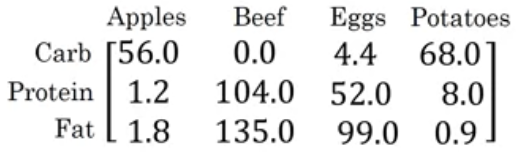
\includegraphics[width=0.38\textwidth]{broadcasting_example.png}
\end{wrapfigure}
\vspace{6pt}

We have briefly used broadcasting in the previous sections to make our code run faster. Let us explore it in a little more detail using the following example. The adjoining matrix contains the number of calories from carbohydrates, proteins and fats per 100g for 4 different foods. Let's say we want to calculate the \% of calories from carbohydrates, proteins and fats for all the 4 foods.  
\vspace{-6pt}

We might start out by summing the calories in individual columns. Then, we would calculate each of the \% respectively by dividing each term by its corresponding total. Using the above vectorization techniques, we can perform the above task in 2 lines of code.
\begin{Verbatim}[tabsize=2]
> import numpy as np
	
	A = np.array([56.0, 0.0, 4.4, 68.0],
							 [1.2, 104.0. 52.0, 8.0],
							 [1.8, 135.0, 99.0, 0.9])
	
	cal = A.sum(axis=0) # axis = 0 --> sum vertically; axis=1 --> sum horizontally
	percentage = 100*A/cal
	
	print(percentage)
\end{Verbatim}
The line \texttt{percentage = 100*A/cal} is an example of broadcasting in python. What we have essentially done is divide a $3\times 4$ matrix by a $1\times 4$ matrix. This type of broadcasting works with both column vectors as well as row vectors. Let's go through another example. If we try to perform the following addition in Python,
$$\begin{bmatrix}
	1 \\
	2 \\
	3 \\
	4 \\
\end{bmatrix} +100\longrightarrow
\begin{bmatrix}
	1 \\
	2 \\
	3 \\
	4 \\
\end{bmatrix}+
\begin{bmatrix}
	100 \\
	100 \\
	100 \\
	100 \\
\end{bmatrix}=
\begin{bmatrix}
	101 \\
	102 \\
	103 \\
	104 \\
\end{bmatrix}$$
We saw this type of broadcasting in our earlier code for logistic regression with the line \texttt{Z = np.dot(w.t,x)+b}.
\subsection{Python and \texttt{numpy} vectors}
The \texttt{numpy} library in Python allows for broadcasting. As we have already seen, this can make our code a whole lot shorter. However, this may also lead to certain hard-to-find bugs in the code if one is not really familiar with how broadcasting works. Some of the most common bugs occur with rank 1 arrays.
\begin{Verbatim}[tabsize=2]
> import numpy as np
	
	a = np.random.randn(5)
	
	print(a.shape)
	print(a) # prints out the array
	print(a.T) # still prints out the same array
	print(np.dot(a,a.T)) # prints a single number instead of a matrix
\end{Verbatim}
The first line prints out \texttt{(5,)}, indicating that the array is of rank 1. This type of data structure does not behaves consistently as either a row vector or as a column vector. Its transpose is the same itself. This can lead to some unexpected results with multiplication, etc. 
\vspace{6pt}

To avoid this, it is better to initialise \texttt{a = np.random.randn(5,1)}. Another alternative is to force the dimension using \texttt{assert(a.shape == (5,1))}. If, for some reason, you end up using a rank 1 array, it can be reshaped as \texttt{a.reshape(5,1)}.

\hrulefill
\begin{center}\textbf{END OF WEEK 2 - MODULE 2}\end{center}
This is the end of the course notes for Week 2. Keep on reading further for the notes from further weeks, or spend some time gaining further insight into the previously discussed topics.

\hrulefill
\pagebreak
\section{Shallow Neural Networks}
In the previous section, we saw how to implement a single iteration of logistic regression, i.e. a neural network with a single node. The node computed 2 variables $z$ and $a$.
\begin{center}
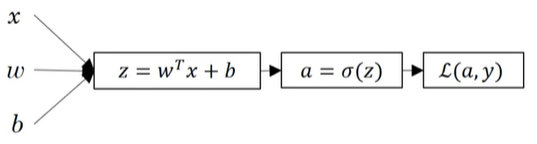
\includegraphics{week2.png}
\end{center}
Most often, neural networks will have multiple nodes distributed between multiple `hidden' layers. Let us see an example of a neural network with one hidden node:
\begin{center}
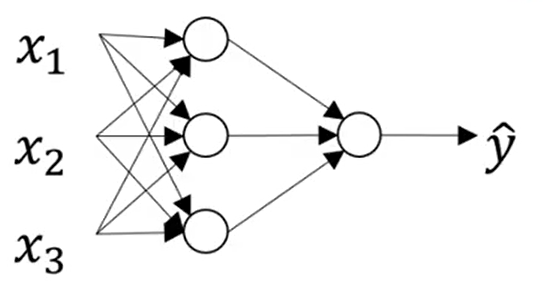
\includegraphics[scale=0.5]{week3.png}
\end{center}
Each of the individual neurons corresponds to a computation of $z$ and $a$:
\begin{itemize}
	\item the first stack of nodes will receive an input as $W^{[1]},b^{[1]},x$$$z^{[1]}=W^{[1]}x+b^{[1]}\longrightarrow a^{[1]}=\sigma(z^{[1]})$$
	\item the second layer (a single node) will receive input $W^{[2]},b^{[2]},a^{[1]}$ from the first layer and follow a similar computation
$$z^{[2]}=W^{[2]}a^{[1]}+b^{[2]}\longrightarrow a^{[2]}=\sigma(z^{[2]})\longrightarrow \Lagr(a^{[2]},y)$$
\end{itemize}
\textbf{NOTE:} The above notation will be used throughout the next sections. This notation $W^{[i]},b^{[i]},a^{[i]}$ corresponds to different layers in the neural network and is not to be confused with $W^{(i)},b^{(i)},a^{(i)}$, which corresponds to individual training examples.
\subsection{Neural network representation}
Now that we have seen the basic representation of a neural network, let us explore a neural network with a single hidden layer in a little more detail. 
\begin{wrapfigure}[11]{L}{0.4\textwidth}
\centering 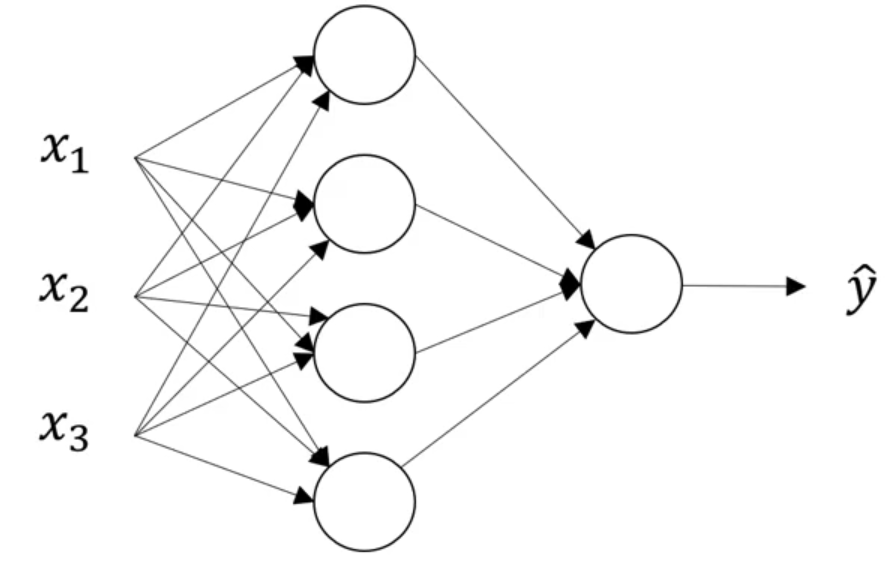
\includegraphics[width=0.38\textwidth]{single_hidden_layer.png}
\end{wrapfigure}
\vspace{6pt}

The input features $x_1,x_2,x_3$ stacked vertically form the input layer of the neural network. Similarly, the final layer (in this case, just a single node) forms the output layer and is responsible for generating the predicted value $\hat{y}$. 
\vspace{6pt}

In the middle, we have the hidden layer of the neural network. The training dataset contains values from both the input layer as well as the output layer. However, the true values for the middle nodes are not observed in the training set, and hence the term `hidden'.
\vspace{6pt}

Let us now introduce a little more notation with reference to the diagram alongside:
\begin{itemize}
	\item initially we used the vector $X$ to denote the input features $\rightarrow$ an alternative notation for the input features is $a^{[0]}=X$
\end{itemize}
The term $a$ stands for activations and refers to the values that different layers in the neural network pass on to subsequent layers.
\begin{itemize}
	\item the next layer will, in turn, generate a set of activations $a^{[1]}=\{a_1^{[1]},a_2^{[1]},a_3^{[1]},a_4^{[1]}\}$
	\item the final layer will generate a value $a^{[2]}$, a real number, which corresponds to $\hat{y}$
\end{itemize}

\subsection{Computing the output of a neural network}
In logistic regression, we had a single node which computed $z=w^Tx+b$ and $a=\sigma(z)$. A neural network just does this a lot more times.
\vspace{6pt}
Consider the first node in the hidden layer of the network in Section 5.1. It computes $z_1^{[1]}={w_1^{[1]}}^Tx+b_1^{[1]}$ and $a_1^{[1]}=\sigma(z_1^{[1]})$. Similarly, the second layer computes $z_2^{[1]}={w_2^{[1]}}^Tx+b_2^{[1]}$ and $a_2^{[1]}=\sigma(z_2^{[1]})$, and so on. Naturally, using a \texttt{for} loop in such a case is inefficient, and even more so when the number of nodes increases. Let's see how we can vectorize the set of 4 equations corresponding to the middle layer. 
\vspace{6pt}

Let's start with computing $z$ as a vector. We define the vector $Z^{[1]}$ and matrices $W^{[1]},B^{[1]}$ as
$$Z^{[1]}=
\begin{bmatrix}
	\cdots & w_1^{[1]T} & \cdots\\
	\cdots & w_2^{[1]T} & \cdots\\
	\cdots & w_3^{[1]T} & \cdots\\
	\cdots & w_4^{[1]T} & \cdots\\
\end{bmatrix}
\begin{bmatrix}
	x_1\\
	x_2\\
	x_3\\
\end{bmatrix} 
 +
\begin{bmatrix}
	b_1^{[1]}\\
	b_2^{[1]}\\
	b_3^{[1]}\\
	b_4^{[1]}\\
\end{bmatrix}= W^{[1]}x+B^{[1]}=
\begin{bmatrix}
	w_1^{[1]T}x+b_1^{[1]}\\
	w_2^{[1]T}x+b_2^{[1]}\\
	w_3^{[1]T}x+b_3^{[1]}\\
	w_4^{[1]T}x+b_4^{[1]}\\
\end{bmatrix}=
\begin{bmatrix}
	z_1^{[1]}\\
	z_2^{[1]}\\
	z_3^{[1]}\\
	z_4^{[1]}\\
\end{bmatrix}
$$
Finally we define another vector $A^{[1]}=\sigma(Z^{[1]})$ which simply stacks up all the values $a_1^{[1]},a_2^{[1]},a_3^{[1]},a_4^{[1]}$. The computation in the final node is very similar, except for a change in the layer index.
\subsection{Vectorization across multiple examples}
The previous section dealt with computing the output of a neural network for a single example. Let's how try to compute the output over an entire training set.
$$x\longrightarrow a^{[2]}=\hat{y} \left\{
\begin{array}{l}
    x^{(1)}\longrightarrow a^{[2](1)}=\hat{y}^{(1)} \\
    x^{(2)}\longrightarrow a^{[2](2)}=\hat{y}^{(2)} \\
    \vdots \\
    x^{(m)}\longrightarrow a^{[2](m)}=\hat{y}^{(m)}\\
\end{array}{}\right.$$
We now have to refine the matrices $Z^{[1]}$ and $A^{[1]}$ so that we vertically span over the number of nodes in the hidden layer and horizontally span across the number of training examples:
$$X=A^{[0]}
\begin{bmatrix}
	\vdots & \vdots & & \vdots\\
	x^{(1)} & x^{(2)} & \cdots & x^{(m)}\\
	\vdots & \vdots & & \vdots\\
\end{bmatrix};
Z^{[1]}=
\begin{bmatrix}
	\vdots & \vdots & & \vdots\\
	z^{[1](1)} & z^{[1](2)} & \cdots & z^{[1](m)}\\
	\vdots & \vdots & & \vdots\\
\end{bmatrix};
A^{[1]}=
\begin{bmatrix}
	\vdots & \vdots & & \vdots\\
	a^{[1](1)} & a^{[1](2)} & \cdots & a^{[1](m)}\\
	\vdots & \vdots & & \vdots\\
\end{bmatrix}
$$
The implementation of this into code is very similar to what we did with logistic regression $-$ only the matrices are of a bigger order. The final vector equations we now have are:
$$Z^{[1]}={W^{[1]}}^TX+b^{[1]}\longrightarrow A^{[1]}=\sigma(Z^{[1]})$$
$$Z^{[2]}={W^{[2]}}^TA^{[1]}+b^{[2]}\longrightarrow A^{[2]}=\sigma(Z^{[2]})$$
\subsection{Activation functions}
An activation function is the function that passes on parameters from one layer of a neural network to the next. For example, in our example, the function $A^{[1]}=\sigma(Z^{[1]})$ is the activation function. Up till now, we have been using the sigmoid function as the activation function. There are many other choices and sometimes, these can work much better.
\vspace{6pt}

Generally we choose non-linear sigmoid functions. We do this because otherwise, $\hat{y}$ would just be a linear computation of the input features. While working with many hidden layers, if the activation function is just a linear combination of the input, it makes the purpose of having multiple layers redundant since the output is so predictable and can just be hardcoded.
\vspace{6pt}

In fact, in our current example, if we use the linear activation function $g(z)=z$ for the hidden layer, then the model is no more expressive that standard logistic regression without any hidden layer.
\vspace{6pt}

We can replace the function $\sigma(Z^{[1]})$ with a different general function $g(Z^{[1]})$ which is non-linear. One example of a function that almost always performs better than the sigmoid is the $\tanh$ function. The formula for the $\tanh$ function is
$$\tanh(z)=\frac{e^z-e^{-z}}{e^z+e^{-z}}$$
It turns out that applying $\tanh$ as the activation function for the middle layer almost always leads to better results than using the sigmoid. This is because, since the values lie between $-1$ and 1, the mean of the data lies closer to 0 than to 0.5. This actually makes the learning for the next layer easier. One exception to when sigmoid would be a more preferable choice is during binary classification, where we want the output predictions to be between 0 and 1.
\vspace{6pt}

One disadvantage of both the sigmoid and tanh function is that for very large and small $z$, the slope of the function ends up very close to 0, which can slow down gradient descent. This brings us to another popular activation function called the ReLU (rectified linear unit).
\begin{wrapfigure}[10]{L}{0.3\textwidth}
\centering 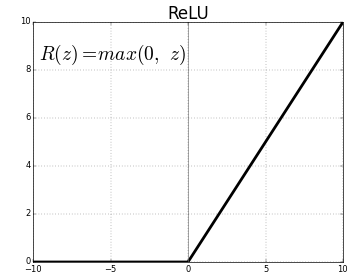
\includegraphics[width=0.28\textwidth]{relu.png}
\end{wrapfigure}
\vspace{6pt}

The ReLU function is defined as $R(z)=\max(0,z)$. Technically, the derivative of this function at $z=0$ is not defined, but the odds of running into the exact case $z=0$ are extremely small. To handle for that case, we can artificially define it to be either 0 or 1 without affecting the accuracy much. The ReLU is increasingly becoming the default choice of activation function. 
\vspace{-6pt}

One disadvantage of the ReLU is that the derivative is zero for all $z<0$. This can be rectified by changing the slope to a very subtle angle $-$ this type of ReLU is called the `leaky' ReLU. However, despite it working better than the ReLU, it is not used as much.
\vspace{18pt}

\textbf{NOTE:} Linear activation functions are usually not preferred in hidden layers, but one of the rare applications of linear activation functions is in compression algorithms. Linear activation functions are also somewhat commonly used in the output layer since the final range of $y$ and $\hat{y}$ are the same.
\subsection{Gradient descent for neural networks}
We have seen how to vectorize the forward propagation steps for out neural network. Let's now get into back propagation using gradient descent, for which we need to first define the gradients of various activation functions. For an activation function $a=g(z)$, with a little bit of calculus, we can prove the following results:
$$g(z)=\sigma(z)=\frac{1}{1+e^{-z}}\longrightarrow g^{\prime}(z)=a(1-a)$$
$$g(z)=\tanh(z)=\frac{e^z-e^{-z}}{e^z+e^{-z}}\longrightarrow g^{\prime}(z)=(1+a)(1-a)$$
$$g(z)=\max(0,z)\longrightarrow g^{\prime}(z)= \left\{
\begin{array}{cc}
	0 & \text{ if } z<0\\
	1 & \text{ if } z>0\\ 
\end{array} \right.$$
$$g(z)=\max(0.01z,z)\longrightarrow g^{\prime}(z)= \left\{
\begin{array}{lc}
	0.01 & \text{ if } z<0\\
	1 & \text{ if } z>0\\ 
\end{array} \right.$$
Note that for the ReLU and leaky ReLU functions we can set the derivative at $z=0$ to be either 0 or 1, without affecting the accuracy of the algorithm much. Now that we have defined the derivatives of the various activation functions, let's get into implementing gradient descent.
\vspace{6pt}

We have the input parameters $X,W^{[1]},b^{[1]},W^{[2]}$ and $b^{[2]}$. Let us define $n^{[1]},n^{[2]}$ as the number of nodes in the hidden layer and the output layer respectively. $X$ is of dimension $(n_x,n^{[1]})$, or $(n^{[0]},n^{[1]})$ for a more consistent notation. The dimensions of 
$W^{[1]},b^{[1]},W^{[2]},b^{[2]}$ are $(n^{[1]},n^{[0]}),(n^{[1]},1),(n^{[2]},n^{[1]}),(n^{[2]},1)$ respectively. Let us assume, for now, that we are performing binary classification. Then, the loss and cost functions will have a very similar form to that we used in case of logistic regression earlier:
$$J(W^{[1]},b^{[1]},W^{[2]},b^{[2]})=\frac{1}{m}\sum_{i=1}^m\Lagr(\hat{y},y)=\frac{1}{m}\sum_{i=1}^m\Lagr(a^{[2]},y)$$
To then carry out gradient descent, we need to compute the gradients $\dfrac{\text{d}J}{\text{d}W^{[1]}},\dfrac{\text{d}J}{\text{d}b^{[1]}},\dfrac{\text{d}J}{\text{d}W^{[2]}},\dfrac{\text{d}J}{\text{d}b^{[2]}}$. After this is done, we would need to update the parameters on each iteration using $$W^{[1]}=W^{[1]}-\alpha\left(\dfrac{\text{d}J}{\text{d}W^{[1]}}\right);b^{[1]}=b^{[1]}-\alpha\left(\dfrac{\text{d}J}{\text{d}b^{[1]}}\right);W^{[2]}=W^{[2]}-\alpha\left(\dfrac{\text{d}J}{\text{d}W^{[2]}}\right);b^{[2]}=b^{[2]}-\alpha\left(\dfrac{\text{d}J}{\text{d}b^{[2]}}\right)$$
Let us finally express the gradient descent algorithm as a bunch of equations (keep in mind that any notation of the form $\text{d}Z^{[1]}$ actually means $\left.\dfrac{\text{d}J}{\text{d}Z^{[1]}}\right)$. We use the sigmoid as the activation function for the output layer, and a function $g^{[1]}(Z^{[1]})$ for the hidden layer.
\begin{center}
\begin{tabular}{c|c}
	\textbf{Forward Propagation} & \textbf{Back Propagation}\\\\	
	$Z^{[1]}={W^{[1]}}^TX+b^{[1]}$ & $\text{d}Z^{[2]}=A^{[2]}-Y$\\\\
	$A^{[1]}=\sigma(Z^{[1]})$ & $\text{d}W^{[2]}=\dfrac{1}{m}\texttt{np.dot(}\text{d}Z^{[2]},{A^{[1]}}\texttt{.T)}$\\\\
	$Z^{[2]}={W^{[2]}}^TA^{[1]}+b^{[2]}$ & $\text{d}b^{[2]}=\dfrac{1}{m}\texttt{np.sum(}\text{d}Z^{[2]}\texttt{,axis=1,keepdims=True)}$\\\\
	$A^{[2]}=\sigma(Z^{[2]})$ & $\text{d}Z^{[1]}=\texttt{np.dot(}W^{[2]}\texttt{.T,}\text{d}Z^{[2]}\texttt{)}\times{g^{[1]}}^{\prime}(Z^{[1]})$\\\\
	 & $\text{d}W^{[1]}=\dfrac{1}{m}\texttt{np.dot(}\text{d}Z^{[1]},X\texttt{.T)}$\\\\
	  & $\text{d}b^{[1]}=\dfrac{1}{m}\texttt{np.sum(}\text{d}Z^{[1]}\texttt{,axis=1,keepdims=True)}$\\\\
\end{tabular}
\end{center}
\subsection{Initialization of variables}
In our implementation of logistic regression, we initialised the variables all to 0. In the case of neural networks, this won't work. Consider a neural network with 2 input features and 2 hidden units.
\begin{wrapfigure}[6]{L}{0.35\textwidth}
\centering 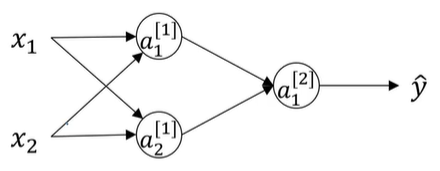
\includegraphics[width=0.33\textwidth]{initialization.png}
\end{wrapfigure}
\vspace{6pt}

Let's say we initialize $W^{[1]},W^{[2]},b^{[1]}$ all to null matrices. It turns out that initialising $b^{[1]}$ to 0 is okay, but it is a problem in case of $W^{[1]}$ and $W^{[2]}$. This is because then, $z_1^{[1]}=z_2^{[1]}\implies a_1^{[1]}=a_2^{[1]}$, since both of the nodes are computing the same activation function. Due to this, during back propagation, we get the result that $\text{d}z_1^{[1]}=\text{d}z_2^{[1]}$. So essentially, the 2 nodes are now identical (or symmetric).
\vspace{6pt}

By mathematical induction over the number of iterations, it can be proven that both the nodes compute exactly the same function during each iteration. Hence, there is really no point to having more than one hidden unit. We want them to be computing different functions.
\vspace{6pt}

A solution to this is to initialize the parameters to random values i.e. $w^{[1]}=\texttt{np.random.randn((2,2))*0.01}$ and so on. We multiply by a small factor to ensure that $w$, hence $z$, and hence $a$ are small enough to not end up on the flat parts of the activation function curve.

\hrulefill
\begin{center}\textbf{END OF WEEK 3}\end{center}
This is the end of the course notes for Week 3. Keep on reading further for the notes from further weeks, or spend some time gaining further insight into the previously discussed topics.

\hrulefill
\pagebreak
\section{Deep Neural Networks}
\textit{(This section is currently in the works. Expect it to be up within a week's time.)}

\hrulefill
\end{document}

